%%================================================
%% Filename: chap04.tex
%% Encoding: UTF-8
%% Author: Yuan Xiaoshuai - yxshuai@gmail.com
%% Created: 2012-04-28 00:15
%% Last modified: 2019-11-06 17:39
%%================================================
\chapter{基于RNM-MF的iCarl增量学习攻击检测及IGPPM溯源系统实现}
\label{cha:ResNet-BiGRU-IGPPM}

% 在现代网络安全领域,快速准确地检测潜在攻击的能力至关重要。
% 但是,我们面临的挑战在于,传统的攻击检测方法往往依赖于预先定义的特征集,这可能导致对新型攻击的检测能力不足,因为它们无法适应不断变化的攻击模式。
% 另外,实际的流量数据有着海量高维的特点,然而常规的算法通常不会针对这种特点进行调整适应,往往结果是生成的模型在实际部署中准确率低、误报率高。
% 因此,为了能够解决这种概念漂移问题和能够有效挖掘复杂网络数据的深层特征以达到更高的检测精度,我们引入了基于特征选择优化的 ResNet-BiGRU 分类检测模型。
% 图~\ref{fig:attack_detecion_model}~描述了我们的检测模型的工作原理和流程。
% \begin{figure}[htbp]
%   \centering
%   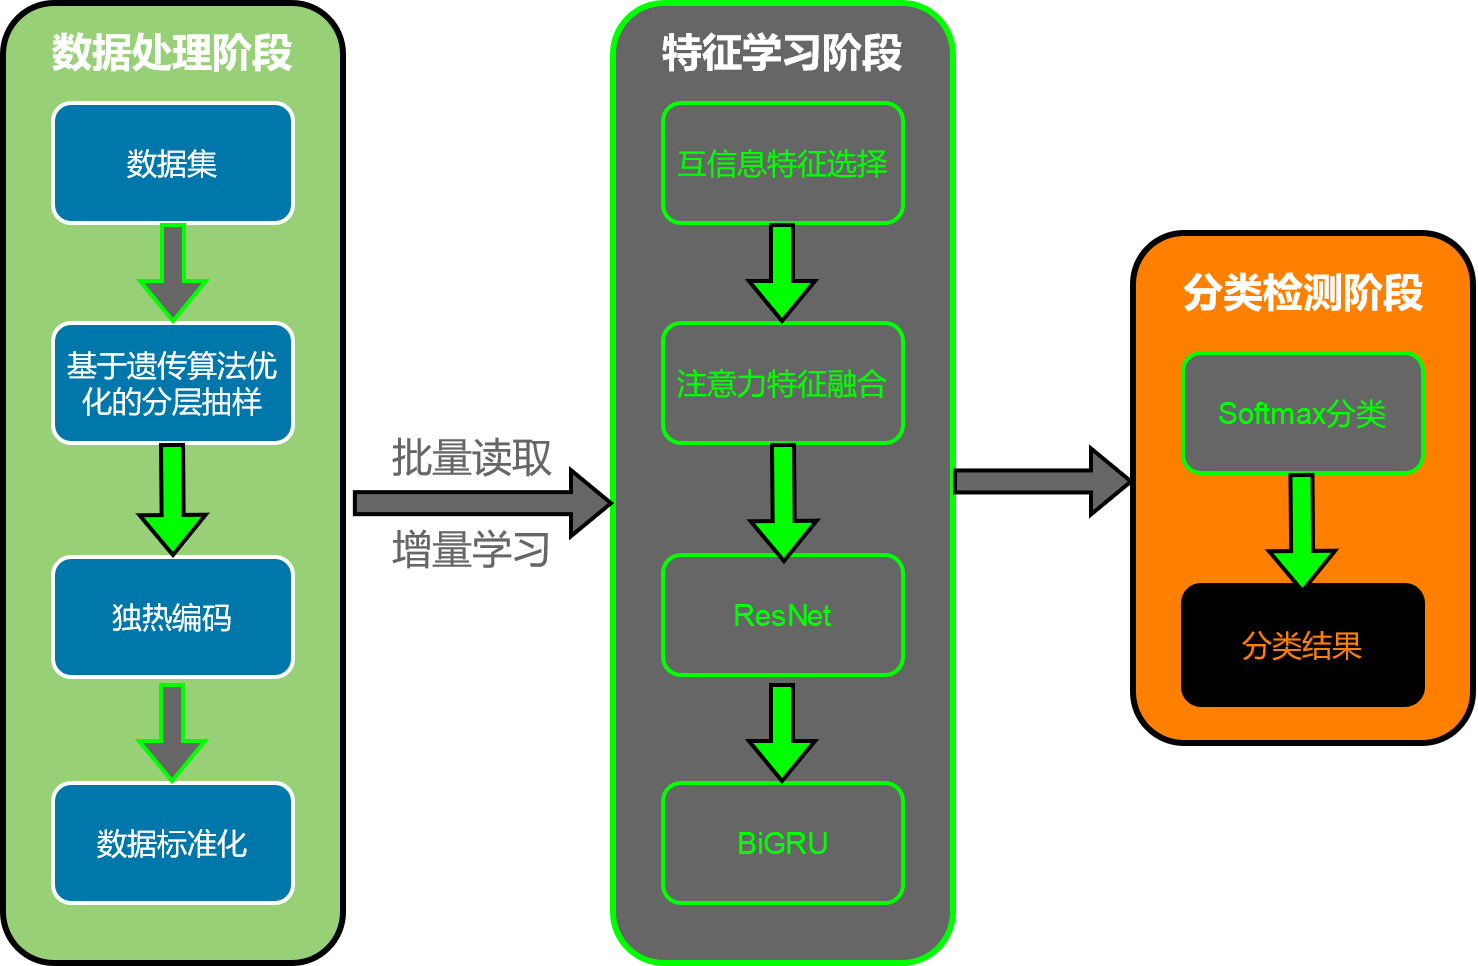
\includegraphics[width = 0.8\textwidth]{ourmodel.drawio.png}
%   \caption{基于特征选择优化的 ResNet-BiGRU 分类检测模型}
%   \label{fig:attack_detecion_model}
% \end{figure}


% 模型首先采用遗传算法对分层抽样过程进行优化,保证训练集的质量;
% 之后利用互信息冗余算法进行特征降维来提高算法效率减少过拟合的风险;
% 训练采用增量学习的方式适应不断变化的攻击模式,减少对数据集的依赖性;
% 最后利用ResNet-BiGRU的优势来解决深度网络中的梯度消失问题、捕捉时间序列数据中的长期依赖关系,从而挖掘复杂网络数据的深层特征,提高检测精度和准确率。
% 接下来,我们将详细地从实验数据集、数据集预处理、模型具体结构设计、实验设置、实验结果逐步展开介绍。
本文第三章设计了基于接口号分组的概率包标记法,第四章设计了基于RNB-MF的网络异常流量检测模型并通过实验验证了其优越性。
继续沿着这一研究方向,本章将会再提出一个基于RNB-MF的iCarL增量学习策略,并结合第三章提出的基于接口号分组的概率包标记法设计一个既能进行网络攻击检测也能支持攻击溯源的增量学习系统。
\section{实验数据集}

\subsection{NSL-KDD数据集\cite{revathi2013detailed}}
KDD Cup 99数据集\cite{tavallaee2009detailed}曾长期被视为网络入侵检测研究的标准化数据集。
然而,该数据集存在一些显著的局限性,例如庞大的数据量和大量的冗余记录,这些因素共同导致了模型训练和测试的效率低下。
为了解决这些问题并提高研究效率,NSL-KDD数据集应运而生,它在网络安全领域得到了广泛的应用和认可。


NSL-KDD数据集的设计考虑到了消除冗余性、改善平衡性、增加多样性和扩展适用性。
通过从原始的KDD Cup 99数据集中移除冗余记录,NSL-KDD显著减少了数据量,从而使得模型和算法能够在较短的时间内完成训练,同时降低了因数据冗余可能引入的偏差风险。
尽管NSL-KDD并未完全解决数据类别不平衡的问题,但相较于其前身,它在一定程度上减轻了这一问题,为研究人员提供了一个更加平衡的数据环境。


NSL-KDD数据集由41个特征组成,整体包括八个文件,分成四组数据,每组提供了两种格式:文本(.txt)和属性关系文件格式(.arff)。
这些文件的详细描述如下表~\ref{tab:NSLKDDFile}~。
\begin{table}[htbp]
  \caption{NSL-KDD数据集各文件介绍}
  \label{tab:NSLKDDFile}
  \begin{tabularx}{\textwidth}{cXc}
    \toprule
    \textbf{文件名} & \textbf{描述} & \textbf{记录总数}\\
  \midrule
    KDDTrain+.ARFF & 完整的NSL-KDD训练集以二进制标签的ARFF格式提供 &125973\\
    KDDTrain+.TXT & 完整的NSL-KDD训练集,包括攻击类型标签和难度级别,以CSV格式提供&125973\\
    KDDTrain+20Percent.ARFF & KDDTrain+.arff文件的20\%子集&25192\\
    KDDTrain+20Percent.TXT & KDDTrain+.txt文件的20\%子集 &25192\\
    KDDTest+.ARFF & 完整的NSL-KDD测试集以二进制标签的ARFF格式提供 &22544\\
    KDDTest+.TXT & 完整的NSL-KDD测试集,包括攻击类型标签和难度级别,以CSV格式提供 & 22544\\
    KDDTest-21.ARFF & 不包含难度级别为21的记录的KDDTest+.arff文件的子集 &11850\\
    KDDTest-21.TXT & 不包含难度级别为21的记录的KDDTest+.txt文件的子集&11850 \\
  \bottomrule
  \end{tabularx}
\end{table}

NSL-KDD数据集中包含的攻击流量可分为拒绝服务攻击(DoS)、远程到本地攻击(R2L)、用户到根攻击(U2R)以及探测攻击(Probe)共四种类别。
如表~\ref{tab:attack_class}~所示,这四种类别又可细分为39种子类型。
表~\ref{tab:kdd_distribution}~则展示四种类别的攻击流量与正常流量在数据集中的分布占比。
图~\ref{fig:kddtraindistribution}~、~\ref{fig:kddtestdistribution}~分别是完整训练集与测试集中各种流量分布占比饼状图。


通过以上图表可知数据集中不同攻击类型的数据分布不均衡,特别是U2R和R2L攻击类型的样本数量远少于其他类型。
这种不平衡分布对于训练入侵检测系统模型来说是一个挑战,因为模型可能会在较多样本的攻击类型上表现更好,而在样本较少的攻击类型上表现不佳。
此外,从KDDTrain+到KDDTest+,攻击类型的分布变化表明,测试集可能代表了与训练集不同的攻击环境,这要求模型具备良好的泛化能力,以适应不同的攻击行为和模式。


\begin{table}[htbp]
  \caption{NSL-KDD数据集中每种攻击的不同子类的细分}
  \label{tab:attack_class}
  \begin{tabularx}{\textwidth}{@{}ccX@{}}
  \toprule
    \multicolumn{1}{c}{\textbf{种类}} & \multicolumn{1}{c}{\textbf{数量}} & \multicolumn{1}{c}{\textbf{子类}}\\
  \midrule
    DoS & 11 & apache2, back, land, neptune, mailbomb, pod, processtable, smurf, teardrop, dupstorm, worm\\
    Probe & 6 & ipsweep, mscan, nmap, portsweep, saint, satan\\
    U2R & 7 & buffer\_overflow, loadmodule, perl, ps, rootkit, sqlattack, xterm\\
    R2L & 15 & ftp\_write, guess\_passwd, httptunnel, imap, multihop, named, phf, sendmail, snmpattack, spy, snmpguess, warezclient, warezmaster, xlock, xsnoop\\
  \bottomrule
  \end{tabularx}
\end{table}

\begin{table}[htbp]
  \caption{每种攻击类型的数据分布}
  \label{tab:kdd_distribution}
  \centering
  \begin{tabular}{ccccccc}
  \toprule
  \textbf{数据集} & \textbf{总数} & \textbf{Normal} & \textbf{DoS} & \textbf{Probe} & \textbf{R2L} & \textbf{U2R}\\
  \midrule
  \multirow{2}{*}{KDDTrain+} & \multirow{2}{*}{125973} & 67343 & 45927 & 11656 & 995  & 52   \\
                             &                          &53.46\%& 36.46\% & 9.25\%&0.79\%&0.04\%\\
  \multirow{2}{*}{KDDTest+} & \multirow{2}{*}{22544} & 9711 & 7636 & 2423 & 2574 & 200\\
                            &                           & 43.08\% & 33.87\%& 10.74\%& 11.42\%&0.89\%\\
  \multirow{2}{*}{KDDTrain+20\%} & \multirow{2}{*}{25192} & 13449 & 9234 & 2289 & 209 & 11\\
                                 &                      & 53.39\% & 36.65\%& 9.09\%& 0.83\%&0.04\%\\
  \bottomrule
  \end{tabular}
\end{table}

  \begin{figure}[htbp]
    \centering
    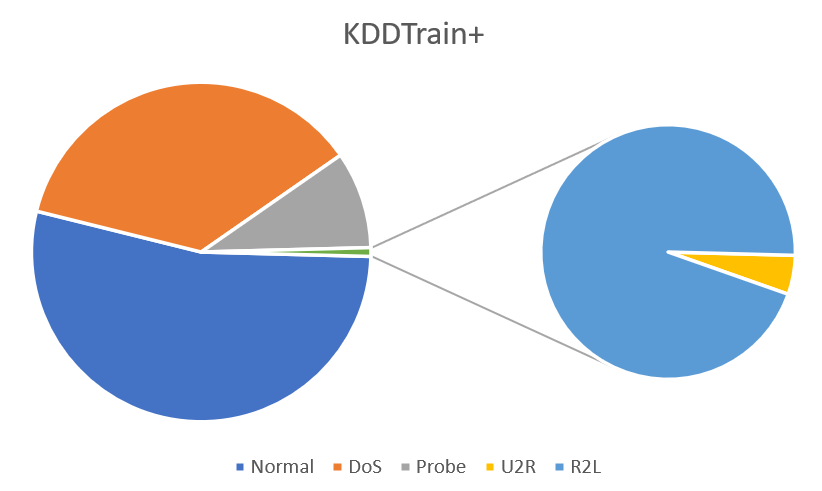
\includegraphics[width = 0.8\textwidth]{kddtraindistribution.png}
    \caption{NSL-KDD完整训练集分类占比饼状图}
    \label{fig:kddtraindistribution}
  \end{figure}

  \begin{figure}[htbp]
    \centering
    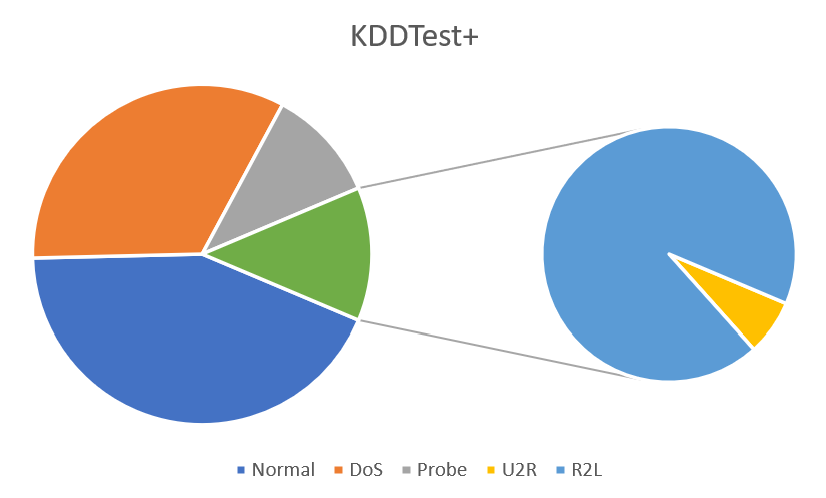
\includegraphics[width = 0.8\textwidth]{kddtestdistribution.png}
    \caption{NSL-KDD完整测试集分类占比饼状图}
    \label{fig:kddtestdistribution}
  \end{figure}


\section{增量学习}
在先前的研究中,我们已经通过实验验证了RNB-MF模型在网络攻击检测任务上的显著性能优势。
具体而言,此模型针对UNSW-NB15数据集中的网络流量数据展现出了卓越的处理效果。
然而,该模型的应用范围受限于其训练数据集的特定特性。
这表明,面对与UNSW-NB15数据集具有本质差异的数据时,模型的表现可能会受到影响。
例如,随着时间推移,新数据的不断累积使得模型需不断适应新增的信息,而旧数据可能因存储限制或隐私保护政策等因素而逐渐失去可用性。
此外,学习任务的复杂度亦可能随之增加,如分类任务中类别数的增长等,而这些变化往往无法事先预定义。\par


\begin{figure}[htbp]
  \centering
  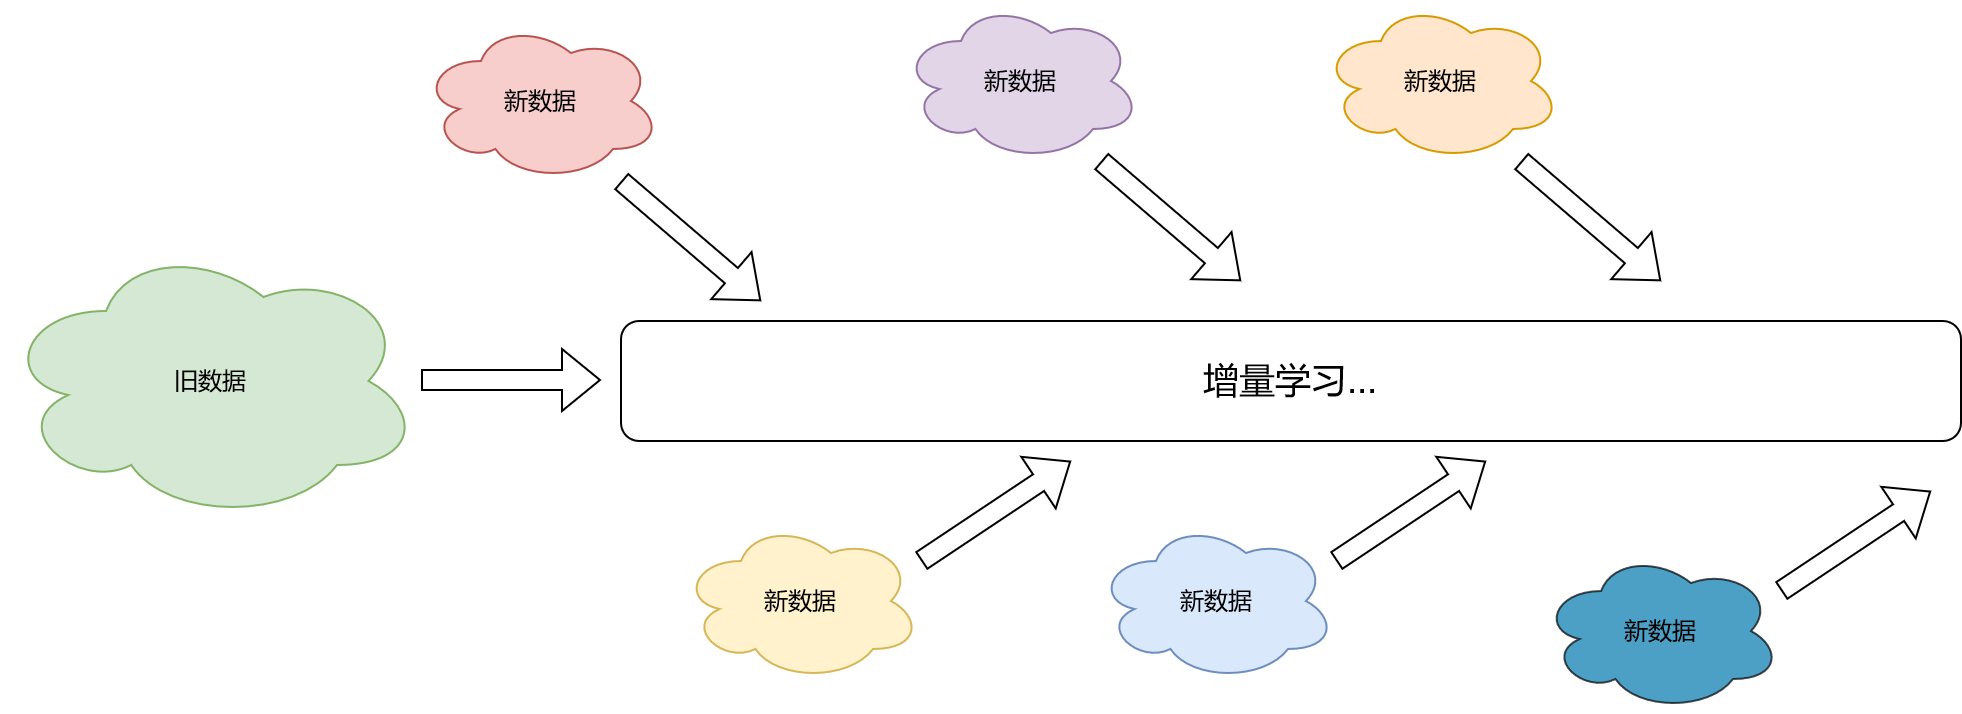
\includegraphics[width=0.8\textwidth]{increment_learning.drawio.png}
  \caption{增量学习原理图}
  \label{fig:incremental_learning}
\end{figure}
因此,探索如何有效地使模型适应新类型的数据,以及如何在数据动态变化的情境下保持模型的稳定性和准确性,成为了重要的研究课题。
针对这一问题,增量学习(Incremental Learning)的概念便成为解决上述问题的一个有效途径。
增量学习(图~\ref{fig:incremental_learning}~)旨在使模型能够逐渐适应新数据或新任务,而无需从头开始重新训练模型。
具体而言,增量学习允许模型在保留已学习知识的基础上,持续地吸收新信息并更新其知识库。

\subsection{基于RNB-MF模型的iCaRL框架}
iCaRL(Incremental Classifier and Representation Learning)\cite{rebuffi2017icarl}是一种经典的基于回放的增量学习策略。
基于回放的增量学习的基本思想就是"温故而知新",即在接受新任务的训练过程中,同时回顾一部分精选的旧数据,以此来保持模型对先前学习任务的记忆。
因此,决定保留哪些旧任务数据以及如何有效地结合旧数据和新数据进行模型训练,是这类方法需要考虑的主要问题。\par


iCaRL的一般步骤为数据特征的学习、记忆集的管理,以及通过知识蒸馏减轻模型的遗忘。
当面对新的数据批次时,iCaRL首先结合这些新数据和从记忆集中选出的代表性样本来更新模型。
记忆集是由每个已知类别中挑选出的一小部分样本构成,旨在代表整个类别的特征分布。
通过在训练过程中包含这些样本,模型可以重新回顾已学习的类别,从而在学习新知识的同时,尽量减少对旧知识的遗忘。
接着,iCaRL通过一个更新的特征提取器来获取数据的特征表示,并利用这些特征来进行分类学习。
在学习新类别的同时,iCaRL使用知识蒸馏(一种让模型学习模仿旧模型输出的方法,详细介绍见~\ref{}~章)来保持对过去学习内容的记忆。
通过将旧模型对同一数据的输出作为额外的训练目标,新模型能够在吸收新信息的同时,减少对旧信息的遗忘。
分类决策在iCaRL中是通过计算样本与每个类别的代表性样本(即记忆集中的样本)的平均特征向量(即类中心见公式\ref{eq:class_means})之间的距离来进行的。
\begin{equation}
  \label{eq:class_means}
  \mu_c = \frac{1}{|P_c|} \sum_{p \in P_c} f(p)
\end{equation}
\begin{flushleft}
  \renewcommand\arraystretch{1.25}
  \begin{tabularx}{\textwidth}{@{}>{\normalsize\rm}l@{\quad}>{\normalsize\rm}l@{——}>{\normalsize\rm}X@{}}
  式中& $\symbf{P_c}$ &表示类别$c$的样本集;\\
  &  $\symbf{f(p)}$&样本$p$的特征表示。\\
  \end{tabularx}\vspace{.5ex}%TODO : 注释内容自动转页接排
\end{flushleft}
分类决策的公式如式~\ref{eq:class_dist}~所示。
\begin{equation}
  \label{eq:class_dist}
  \hat{y} = \arg\min_{c \in C} \|f(x) - \mu_c\|_2
\end{equation}
\begin{flushleft}
  \renewcommand\arraystretch{1.25}
  \begin{tabularx}{\textwidth}{@{}>{\normalsize\rm}l@{\quad}>{\normalsize\rm}l@{——}>{\normalsize\rm}X@{}}
  式中& $\symbf{\hat{y}}$ &表示预测的类别;\\
  &  $\symbf{|f(x) - \mu_c|_2}$&测试样本特征表示与类别$c$的类中心之间的欧氏距离。\\
  \end{tabularx}\vspace{.5ex}%TODO : 注释内容自动转页接排
\end{flushleft}
这种基于最近中心的方法简单有效,因为它直接使用了模型学习到的特征表示来进行类别的判断。

最后,更新记忆集是iCaRL算法中一个至关重要的步骤。
随着新类别的加入,算法必须在有限的记忆容量中做出取舍,选择哪些样本继续保留在记忆集中。
这通常会涉及到对每个类别进行均衡的考虑,确保模型能够公平地回顾所有已知类别,而不是偏向于某些特定的类别
(针对此问题本文接下来将会提出一种基于遗传算法的记忆集抽样优化方法。)

基于此策略,本文接下来会将前章提出的RNB-MF模型整合到iCaRL框架中,进而赋予其增量学习的能力。
融合RNB-MF模型的iCaRL策略实现伪代码如表~\ref{tab:RNB-MF-icarl}所示。
\begin{table}[htbp]
   \caption{融合RNB-MF模型的iCaRL}
   \label{tab:RNB-MF-icarl}
   \centering
   \begin{tabularx}{1.0\textwidth}{cl}
   \toprule
   \multicolumn{2}{l}{\textbf{融合RNB-MF模型的iCaRL策略实现}}\\
   \midrule
   \multicolumn{2}{l}{\textbf{输入}: 训练序列中的一系列数据集 $\{D_1, D_2, ..., D_n\}$,每个类别保留的样本数 $m$} \\ 
   \multicolumn{2}{l}{\textbf{输出}: 训练好的RNB-MF特征提取器 $f_{\theta}$,更新后的记忆集 $M$} \\
   1& 初始化记忆集 $M$ 为空 \\
   2& 初始化RNB-MF特征提取器 $f_{\theta}$ \\
   3& $for$ 每个新的数据集 $D_t$: \\
   4&\quad \textbf{a.合并新数据集和记忆集:}\\
   5&\quad\quad $D'_t = D_t \cup M$ \\
   6&\\
   7&\quad \textbf{b.使用}$\symbf{D'_t}$\textbf{训练特征提取器网络}$\symbf{f_{\theta}}$\textbf{:}\\
   8&\quad\quad 如果 $t > 1$,即不是处理第一个数据集: \\
   9&\quad\quad\quad i.使用$f_{\theta}$的旧版本对$x$进行前向传播,得到旧类别的输出$logits_{old}$\\
   10&\quad\quad\quad ii.使用知识蒸馏损失和分类损失来更新 $f_{\theta}$: \\
   11&\quad\quad\quad\quad $L = (1 - \alpha) L_{CE} + \alpha L_{KD}$ \Comment{L:整体损失,$L_{CE}$:蒸馏损失,$L_{KD}$:标准交叉熵损失}\\
   12&\quad\quad 否则,如果是处理第一个数据集: \\
   13&\quad\quad\quad 仅使用分类损失来训练 $f_{\theta}$ \\
   14&\\
   15&\quad \textbf{c.更新记忆集} $M$\textbf{:} \\
   16&\quad\quad $for$ 每个类别 $c=1$ 到 $n$: \\
   17&\quad\quad\quad i.从属于类别$c$的数据集$D_c$中提取所有样本$\{x_1, x_2, ..., x_k\}$ \\
   18&\quad\quad\quad ii.使用当前的特征提取器网络$f_{\theta}$计算每个样本的特征表示 \\
   19&\quad\quad\quad iii.计算类别$c$的特征均值向量$\mu_c$\\
   20&\quad\quad\quad vi.选择$m$个样本存入$M$,基于样本对特征空间的覆盖范围\\
   21&\\
   22&\quad\textbf{d.更新分类器:} \\
   23&\quad\quad 对于记忆集$M$中的每个类别$c$: \\
   24&\quad\quad\quad 计算类别$c$的特征表示的均值(类中心)$\mu_c$\\
   25&\quad\quad 当需要对新样本$x$进行分类时:\\
   26&\quad\quad\quad i.使用$f_{\theta}$计算x的特征表示$f(x)$\\
   27&\quad\quad\quad ii.计算$f(x)$与每个类中心$\mu_c$之间的距离\\
   28&\quad\quad\quad iii.将$x$分类到距离最近的类中心所代表的类别\\
   \bottomrule
   \end{tabularx}
  \end{table}
\subsection{基于遗传算法的记忆集优化抽样}
% 在数据集预处理过程中,数据抽样操作是一项关键步骤,尤其在处理大规模数据集时。
% 它不仅能帮助减少计算资源的消耗,还能在一定程度上避免模型过拟合。
% 数据抽样通常被用来从一个大型数据集中选取一个代表性的子集,以进行更为快速和高效的分析。\par
% 数据抽样的基本目标是确保选取的样本能够尽可能地反映出总体数据的特性,包括数据的分布、均值、方差等统计属性。
% 抽样方法大致可以分为两大类:\textbf{概率抽样}和\textbf{非概率抽样}。\par

% 在概率抽样中,每个样本被选中的概率是已知的,这保证了样本的代表性。
% 概率抽样的方法包括简单随机抽样、系统抽样、分层抽样和簇抽样等。
% 在非概率抽样中,样本的选择依赖于研究者的主观判断,而非随机机制,因此每个样本被选中的概率是未知的。
% 常见的非概率抽样方法包括方便抽样、判断(或目的性)抽样和配额抽样等。\par


% \textbf{分层抽样}是一种高效的概率抽样技术,特别适用于处理不均衡数据集。
% 这种方法的核心优势在于它确保了数据集中所有关键的子群体在样本中都能得到适当的代表性。
% 在不均衡数据集的情况下,少数类别的样本容易在随机抽样过程中被遗漏,尤其是当这些类别的样本数量极少时。
% 分层抽样通过保障这些少数类别在样本中的充分代表性,显著提升了模型对这些类别的识别能力。\par

% 此外,分层抽样通过确保样本中所有相关子群体的均匀分布,有助于降低样本的方差,进而提高估计的准确性。
% 这一点对于不均衡数据集尤为重要,因为少数类别对模型的整体性能可能产生显著影响。
% 通过在训练过程中考虑到数据集中的所有子群体,分层抽样促进了模型的泛化能力,使模型能够更有效地处理现实世界数据的多样性与复杂性。
% 通过图~\ref{fig:kddtraindistribution}、\ref{fig:kddtestdistribution}和\ref{fig:UNSW-NB15barchart}~明显可以看出,本文采用的数据集是非常不均衡的,因此本文将会使用分层抽样对数据集进行处理。
% 然而对于分层抽样的最佳比率,却不能通过直观的获取到。为了取得最优的抽样比率,本文将会利用遗传算法对分层抽样进行优化。
% 对于遗传算法,本文已在第~\ref{eq:GA}~章介绍,这里不再赘述,只给出具体实施细节。\par

% \textbf{分层抽样}是一种高效的概率抽样技术,特别适用于处理不均衡数据集。
% 这种方法的核心优势在于它确保了数据集中所有关键的子群体在样本中都能得到适当的代表性。
% 在不均衡数据集的情况下,少数类别的样本容易在随机抽样过程中被遗漏,尤其是当这些类别的样本数量极少时。
% 分层抽样通过保障这些少数类别在样本中的充分代表性,显著提升了模型对这些类别的识别能力。\par

% 此外,分层抽样通过确保样本中所有相关子群体的均匀分布,有助于降低样本的方差,进而提高估计的准确性。
% 这一点对于不均衡数据集尤为重要,因为少数类别对模型的整体性能可能产生显著影响。
% 通过在训练过程中考虑到数据集中的所有子群体,分层抽样促进了模型的泛化能力,使模型能够更有效地处理现实世界数据的多样性与复杂性。
% 通过图~\ref{fig:kddtraindistribution}、\ref{fig:kddtestdistribution}和\ref{fig:UNSW-NB15barchart}~明显可以看出,本文采用的数据集是非常不均衡的,因此本文将会使用分层抽样对数据集进行处理。
% 然而对于分层抽样的最佳比率,却不能通过直观的获取到。为了取得最优的抽样比率,本文将会利用遗传算法对分层抽样进行优化。


在进行增量学习的过程中,每当遇到新的流量类别时,模型就必须在有限的记忆空间内作出取舍。
这就需要确定每个类别的样本在记忆集中应保留的数量或比例,因此对记忆集内各类样本的有效抽样变得十分关键。
虽然传统的iCaRL策略倾向于采用均衡抽取的方法,即平等地从各个类别中抽取样本以保持类别间的平衡,但这种方法并不总能保证模型训练后的分类效果达到最佳。
这是因为不同类别的样本对于模型学习的贡献度并不相同,简单的均衡抽样可能无法充分考虑到样本对模型性能的实际影响。

针对这一问题,本小节提出了采用遗传算法优化的抽样策略。
遗传算法是一种模拟自然选择和遗传机制的搜索算法,它通过迭代进化找到问题的最优解。
在iCaRL的上下文中,遗传算法被用来优化记忆集中各个类别样本的保留比例,目标是在有限的记忆空间内最大化模型的分类性能。
对于遗传算法,本文已在第~\ref{eq:GA}~章介绍,这里不再赘述,只给出具体实施细节。\par

(1) 遗传算法的选择\par
遗传算法的种类以及策略多种多样,在这里我们选择采用稳态遗传算法(Steady State Genetic Algorithm, SSGA)作为优化策略。
与传统的遗传算法相比,稳态遗传算法的特点在于每次迭代只替换种群中的一小部分个体,而不是进行全种群的更新。
这种方法的优势在于绝大多数个体在迭代过程中保持不变,从而避免了每次迭代都进行完整的种群更换。\par

考虑到本文中个体适应度评估的复杂性——每个个体的评估需要经过完整的模型训练及性能评估过程——采用标准遗传算法(即采用完全生成替换策略的遗传算法,其中每次迭代都替换整个种群)将显著增加计算负担,并可能不利于优良基因的保留。
相反,稳态遗传算法通过每次只替换部分种群的策略,不仅大幅度降低了计算量,而且有助于保持种群中的优秀个体。
这种策略的实施有助于加速算法的收敛过程,并且,通过有效地保留高质量的解,稳态遗传算法能够在全局搜索和局部搜索之间取得更好的平衡,从而提高发现全局最优解的可能性。

(2) 特征编码\par
本文使用遗传算法搜索的目标是确定每个类别的样本在记忆集中应保留的数量或比例以便模型能够达到最佳分类效果。
为了实现这一目标,本文将会利用样本类型的抽样比重来进行特征编码。
遗传算法的每个个体(或称为“染色体”)代表一种可能的样本选择方案,其中包含了对应于数据集中每种样本类型的抽样比重。
这些比重被编码为位于$[0,1)$区间的小数,分别表示各类型样本在总体抽样策略中的比重。
以UNSW-NB15数据集为例,一个可能的染色体编码可以是{0.2, 0.3, 0.1, 0.5, 0.3,0.1,0.2,0.1,0.4,0.1},这分别对应于十种样本类型的采样比重。
需要注意的是,这些比重在实际应用中将会具体调整为抽样百分比。
在进行实际训练时,通过计算训练集样本数量与各类样本抽样百分比的乘积,便可得到每类样本具体的抽样数量。
例如,对于样本数量为100,000的数据集,该染色体对应的每类样本采样百分比、采样数量如表~\ref{tab:Ga_code}~所示。\par

\begin{table}
  \caption{遗传算法编码方案}
  \label{tab:Ga_code}
  \centering
  \begin{tabular}{cccc}
    \toprule
    \textbf{编码值(基因)}&\textbf{样本类型}&\textbf{采样百分比}&\textbf{抽样数量}\\
    \midrule
    0.2&normal&8.695652\%&8696\\
    0.3&Fuzzers&13.043478\%&13043\\
    0.1&Reconnaissance&4.347826\%&4348\\
    0.5&Shellcode&21.73913\%&21739\\
    0.3&Analysis&13.043478\%&13043\\
    0.1&Backdoors&4.347826\%&4348\\
    0.2&DoS&8.695652\%&8696\\
    0.1&Exploits&4.347826\%&4348\\
    0.4&Generic&17.391304\%&17391\\
    0.1&Worms&4.347826\%&4348\\
    \bottomrule
  \end{tabular}
\end{table}

(3) 适应度评估\par
在本文中将会利用基因对应的抽样比率对训练集进行分层抽样,并利用RNB-MF模型在增强后的训练集上进行训练。
最后再在验证集上使用accuracy\_score(公式~\ref{eq:val_score1}~)作为评价标准进行评估,评估值便作为该染色体对应的适应度。\par

(4) 初始群体生成及迭代次数\par
为了确保算法能够充分探索解空间并增加解的多样性,我们特别注重初代种群基因的广泛性和迭代过程的深入性。
基于此目的,初始种群规模被设定为1,000个个体。
这一较大的初始种群规模有助于覆盖更广泛的解空间,从而提高找到全局最优解的概率。
同时,为了充分优化解并观察算法的收敛行为,设置了10,000次的迭代次数,以便于算法有足够的时间逐步改进解,并最终接近最优解。\par

% \begin{table}[htbp]
%   \caption{遗传算法实现}
%   \label{tab:genetic_algorithm}
%   \centering
%   \begin{tabularx}{1.0\textwidth}{cl}
%   \toprule
%   \multicolumn{2}{l}{\textbf{遗传算法}}\\
%   \midrule
%   \multicolumn{2}{l}{\textbf{输入}: 种群大小 $P$,基因数量 $G$,代数 $N$,变异率 $M$} \\
%   \multicolumn{2}{l}{\textbf{输出}: 适应度最高的染色体} \\
%   1& 初始化种群 $pop$ \\
%   2& \textbf{for} 每一代 \textbf{in} $N$: \\
%   3&\quad 计算种群中每个个体的适应度: \\
%   4&\quad\quad 依据染色体基因对应得抽样比率进行分层抽样组成训练集\\
%   5&\quad\quad 利用此训练集对模型进行训练\\
%   6&\quad\quad 将训练好的模型在测试集上进行评估取得准确率作为适应度 \\
%   7&\quad 依据染色体适应度对应的概率采用轮盘赌方法选择两个父代 $p1$ 和 $p2$ \\
%   8&\quad 通过 $crossover(p1, p2)$ 生成两个后代 $c1$ 和 $c2$  \\
%   9&\quad 对 $c1$ 和 $c2$ 进行 $mutate$ 操作 \\
%   10&\quad 将 $c1$ 和 $c2$ 加入到 $pop$ 中 \\
%   11&\quad 再次计算种群中新进个体的适应度 \\
%   12&\quad 根据适应度计算每个个体的淘汰概率,适应度越小淘汰概率越大 \\
%   13&\quad 依据淘汰概率采用轮盘赌方法淘汰两个个体 \\
%   14& \textbf{return} 适应度最高的染色体 \\
%   \bottomrule
%   \end{tabularx}
% \end{table}

\begin{table}[htbp]
   \caption{遗传算法实现}
   \label{tab:genetic_algorithm}
   \centering
   \begin{tabularx}{1.0\textwidth}{cl}
   \toprule
   \multicolumn{2}{l}{\textbf{遗传算法}}\\
   \midrule
   \multicolumn{2}{l}{\textbf{输入}: 种群大小 $P$,基因数量 $G$,代数 $N$,变异率 $M$} \\
   \multicolumn{2}{l}{\textbf{输出}: 最优染色体} \\
   1& 初始化种群(population) \\
   2& \textbf{for} generation \textbf{in} $N$: \\
   3&\quad \textbf{for} individual \textbf{in} population: \\
   4&\quad\quad \#依据个体基因对应的抽样比率进行抽样\\
   5&\quad\quad train\_set = sampling(train\_set,gene)\\
   6&\quad\quad train(model, train\_set) \\
   7&\quad\quad fitness = evaluate(model, test\_set) \\
   8&\quad \#根据个体适应度利用轮盘赌选择法进行选择\\
   9&\quad $p1, p2$ = select\_parents(population, fitness) \\
   10&\quad $c1, c2$ = crossover($p1, p2$) \\
   11&\quad mutate($c1$), mutate($c2$) with rate $M$ \\
   12&\quad add $c1, c2$ to population \\
   13&\quad update\_fitness(population) \\
   14&\quad \#根据个体适应度对应的淘汰概率利用轮盘赌选择法进行淘汰\\
   15&\quad eliminate\_individuals(population,fitness) \\
   16& \textbf{return} highest\_fitness\_chromosome(population) \\
   \bottomrule
   \end{tabularx}
  \end{table}

(5) 选择、交叉和变异\par
对于选择策略,本文采用轮盘赌选择法,该方法根据个体适应度相对于总体适应度的比例来分配选择概率。
这种方法的优势在于能够有效保证高适应度个体被优先选择,从而引导种群朝着更优解空间方向进化。
在交叉操作方面,为了降低计算的复杂度,本文选择了单点交叉方法。
对于变异策略,本研究设置了0.1的固定概率对新生成的个体中的所有基因进行变异。
在确定变异位置后,以相等的概率选择将该基因值进行1.2倍的放大或0.8倍的缩小。
这样做的目的是保证个体的基因以较小的变化幅度进行细微调整,增强种群的探索能力,同时避免过大的变异导致优秀基因的丢失。
表~\ref{tab:genetic_algorithm}~是我们遗传算法实现的伪代码。






\section{实验评估与分析}
\subsection{实验环境}
为了评估本文所提方案的有效性,本文将利用python语言来实现以上流程,并选用表~\ref{tab:env_setting}~中的配置来进行实验。
\begin{table}[htbp]
  \caption{实验设备配置}
  \label{tab:env_setting}
  \centering
  \begin{tabular}{ccc}
    \toprule
    \textbf{环境类别} & \textbf{设备项目} & \textbf{项目参数}\\
    \midrule
    \multirow{6}{*}{硬件环境}& CPU型号 & Intel(R) Core(TM) i7-11800H\\
                            & CPU规格 & 8核16线程@2.30GHz\\
                            & GPU型号 & NVIDIA GeForce RTX 3060 Laptop GPU\\
                            & 内存大小& 16.0 GB\\
                            & 硬盘类型& SSD\\
                            & 硬盘大小& 1TB\\
                            \hline
    \multirow{3}{*}{软件环境}&操作系统&Windows 11\\
                            &开发语言&Python 3.11.7\\
                            &编辑器 &Visual Studio Code\\                       
    \bottomrule
  \end{tabular}
\end{table}

\subsection{遗传算法优化的分层抽样实验评估}
\begin{figure}[htbp]
  \centering
  
  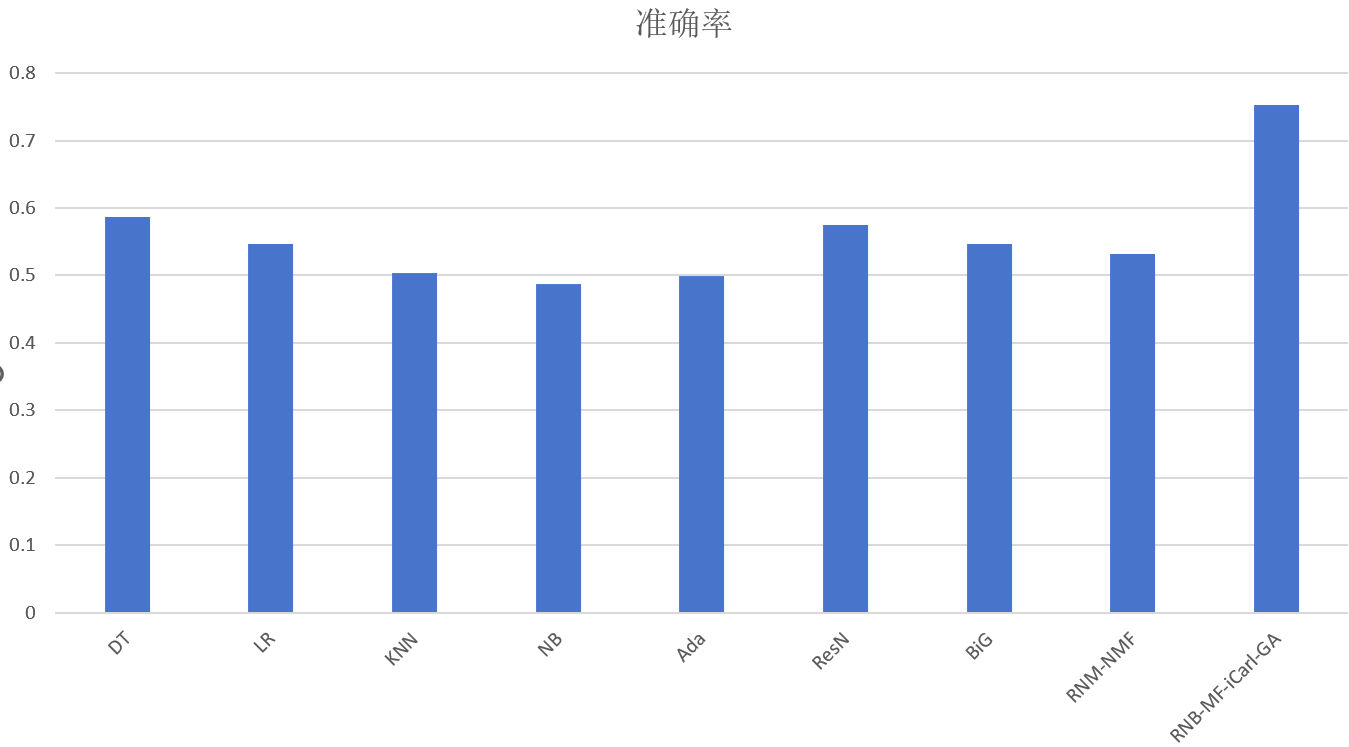
\includegraphics[width=0.8\textwidth]{accuracy_incremental.png}
  \caption{增量学习准确率对比柱状图}
  \label{fig:acc_icarl}
\end{figure}

\section{基于RNM-MF的iCarl增量学习攻击检测及IGPPM溯源系统实现}
